\documentclass[reprint,amsmath,amssymb,aps]{revtex4-2}


\usepackage{graphicx}
\usepackage{amsmath,amssymb,amsfonts}
\usepackage{dcolumn}
\usepackage{bm}
\usepackage{siunitx}
\sisetup{separate-uncertainty=true}
\usepackage[colorlinks,allcolors=blue]{hyperref}
\usepackage{cleveref}
\crefname{equation}{}{}
\crefname{figure}{Fig.}{Figs.}
\crefname{table}{Table}{Tables}
\usepackage{svg}

\begin{document}
\title{Relationship between Newton’s second law and acceleration, mass, and force}
\author{Nitika Kishore}
\email{Contact author: 426nkishore@frhsd.com}
\author{Sameera Patil}
\author{Anton Lavrenov}
\author{Connor Paszkiewicz}
\affiliation{Science \& Engineering Magnet Program, \href{https://manalapan.frhsd.com/}{Manalapan High School}, Englishtown, NJ 07726 USA}
\date{\today}

\begin{abstract}
Using a pulley system with two different masses on either end, this experiment focuses on the relationship between force and acceleration, taking into account various masses. Via the experiment results, we found that Newton’s second law, $\sum F = ma$, was consistent with our measurements. 
\end{abstract}

\keywords{keywords here}

\maketitle
  
\section{Introduction}
Newton's second law of motion is $\sum F=ma$ \cite{tipler}, which states that the force is directly proportional to acceleration. If a force is applied to an object and a force of equal magnitude is applied to a second object, then the object with more mass will accelerate less \cite{tipler}. Furthermore, Newton’s second law states that as acceleration increases, mass should decrease and vice versa. Our goal throughout this experiment was to test how accurate that is by changing various masses used in our cart-pulley system. If Newton’s second law is accurate, $F=ma$ should always stay accurate and constant. We hypothesize that the acceleration should decrease as the masses increase. We also hypothesize that the force of the system ($F=ma$) should stay constant as the weight values on the cart changes. 






\section{Materials and methods}
Our method of testing Newton’s Second Law consisted of a pulley system, where there were two weights: one hanging weight as well as a weight on the cart above (see \cref{fig:1}). Our hanging weight was \qty{0.5}{\kilo\gram} and our weights on the cart (\qty{0.5}{\kilo\gram}) varied between \qty{1.2}{\kilo\gram}, \qty{2.4}{\kilo\gram}, and \qty{3.6}{\kilo\gram}. Our method for measuring acceleration was timing how fast it took our cart to travel \qty{0.50}{\meter} once released using a measuring tape and stopwatch. We assumed that the friction caused by our plane and pulley were negligible. We conducted multiple trials, changing the weights on the cart for each one. We then found acceleration using the formula
\begin{equation}
a = \dfrac{m_{hang}}{m_{cart}+m_{hang}+0.5} g,
\label{eq:apred}
\end{equation}
where $a$ is acceleration, $m_{hang}$ is the hanging mass, $m_{cart}$ is the mass added to the cart, and \qty{0.5}{\kilo\gram} is the cart's empty mass). Finally, we found the forces acting on the system per trial using $\sum F = ma$.

\begin{figure}
\begin{center}
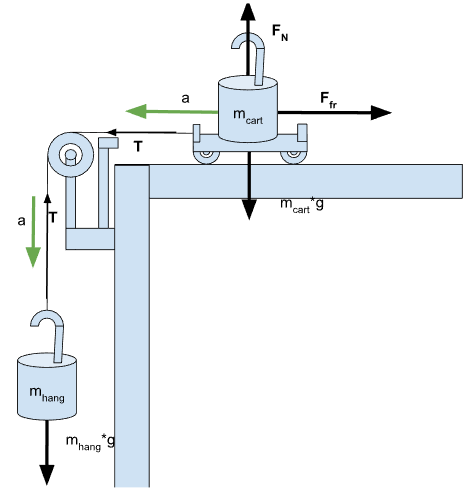
\includegraphics[width=0.66\columnwidth]{fig1.png}
\end{center}
\caption{Experiment Setup FBD}
\label{fig:1}
\end{figure}


\section{Results}
\Cref{tab:newtable1} gives the measured time and resulting acceleration for each value of $m_1$. 
% latex table generated in R 4.4.2 by xtable 1.8-4 package
% Sat Nov 30 16:44:39 2024
\begin{table}
\caption{\label{tab:newtable1} Table caption here.}
\begin{center}
\begin{ruledtabular}
\begin{tabular}{ccc}
$m_1$, \unit{\kilo\gram} & $t$, \unit{\second} & $a$. \unit{\meter\per\second\squared} \\ 
\colrule
1.200 & 0.87 & 1.32 \\ 
2.400 & 1.23 & 0.66 \\ 
3.600 & 1.35 & 0.55 \\ 
\end{tabular}
\end{ruledtabular}
\end{center}
\end{table}

%  Data
%Trial
%	Hanging Mass (kg)
%	Cart Mass (kg)
%	Net Force (N) 
%	Distance (m) 
%	Acceleration  (m/s²) 
%	Time (s)
%	1
%	0.5
%	1.2
%	4.905
%	0.50
%	2.22
%	0.87
%	2
%	0.5
%	2.4
%	4.905
%	0.50
%	1.44
%	1.23
%	3
%	0.5
%	3.6
%	4.905
%	0.50
%	1.06 
%	1.35
%	
%
%                                Total mass (kg) 
\Cref{fig:2} shows a plot of the results from \cref{tab:newtable1} as black dots. The predicted acceleration from \cref{eq:apred} is shown as a blue line. The measured and predicted accelerations agree well. 
\begin{figure}
\begin{center}
\includesvg[width=\columnwidth]{fig2.svg}
\end{center}
\caption{Total Mass (\unit{\kilo\gram}) x Acceleration (\unit{\meter\per\second\squared})}
\label{fig:2}
\end{figure}


\section{Discussion}
\Cref{fig:2} shows that as mass increases, the rate at which acceleration decreases becomes smaller. This correlates with our hypothesis as acceleration is inversely proportional to the total mass in our setup. Despite the changing variables, net force was able to remain constant throughout the entire experiment, supporting our hypothesis that Newton’s second law is always true and consistent. 

\subsection{Sources of experimental error}
Variability in force of the system could be due to friction and how it affects acceleration as well, as we assumed it was negligible. Human error occurring during the timing of the experiment could have also affected our results and in turn, the force of the system. 

\section{Acknowledgments}
We thank several anonymous reviewers for comments that improved the manuscript. We also thank Manalapan High School for providing us with all the materials used throughout this experiment. 

NK timed the experiment, and worked on experiment set-up, original lab report design, and final revisions, AL performed analysis of the data and the figures. CP worked on original lab report revisions and documentation of initial data collection. SP worked on initial lab experiment report design, abstract and conclusion, and the description of the procedure. 




%References
%[1] P. Tipler, G. Mosca, Physics for Scientists and Engineers, Extended (W.H. Freeman and Company, United States, 2004).
%\bibliographystyle{abbrvnat}
\bibliography{lab.bib}
\end{document}

